Final State Radiation (FSR) photons emitted by leptons are not included at all in the Particle Flow reconstruction of muon momentum, and may be missed in electron reconstruction, leading to a degradation of the accuracy for the Z bosons momentum and mass.
The algorithm to select FSR photons is explained in
\todo{cite{HiggsAN}}.

FSR candidates are required to have $p_{T}^{\gamma} >$ 2 GeV, $|\eta^{\gamma}| <$ 2.4, relative isolation $<$ 1.8 (see Equation \ref{eqn:mupfiso}) and $\Delta R(\ell, \gamma) <$ 0.5 with respect to the nearest signal lepton.
Because the electron reconstruction algorithm already recovers some of the FSR photons, we exclude those that have $\Delta R(e, \gamma) <$ 0.15 or $|\Delta\phi(e, \gamma)| <$ 2 and $|\Delta\eta(e, \gamma)| <$ 0.05 to avoid double counting.
Since FSR photons tend to have higher energies than the ones from pileup, and are expected to be quasi-collinear with the emitting leptons, an FSR candidate is accepted if $\Delta R(\ell, \gamma)^{} / E_{T,\gamma}^{2} <$ 0.012 GeV$^{-2}$.
Accepted FSR photons have their momentum added to the lepton and are excluded from the computation of its isolation.
\\
Since our analysis selection requires signal photons to have at least $\Delta R(\ell, \gamma) > 0.5$ from any signal lepton, there is no double counting.
However, we studied the kinematic distributions of photons passing all the other basic kinematic selections with this cut relaxed.
For example, their distribution in bins of $\Delta R(\ell, \gamma)$ with respect to the closest lepton
can be seen in Figure \ref{fig:dRl_fsr_photons}.
\begin{figure}[ht]
\begin{center}
        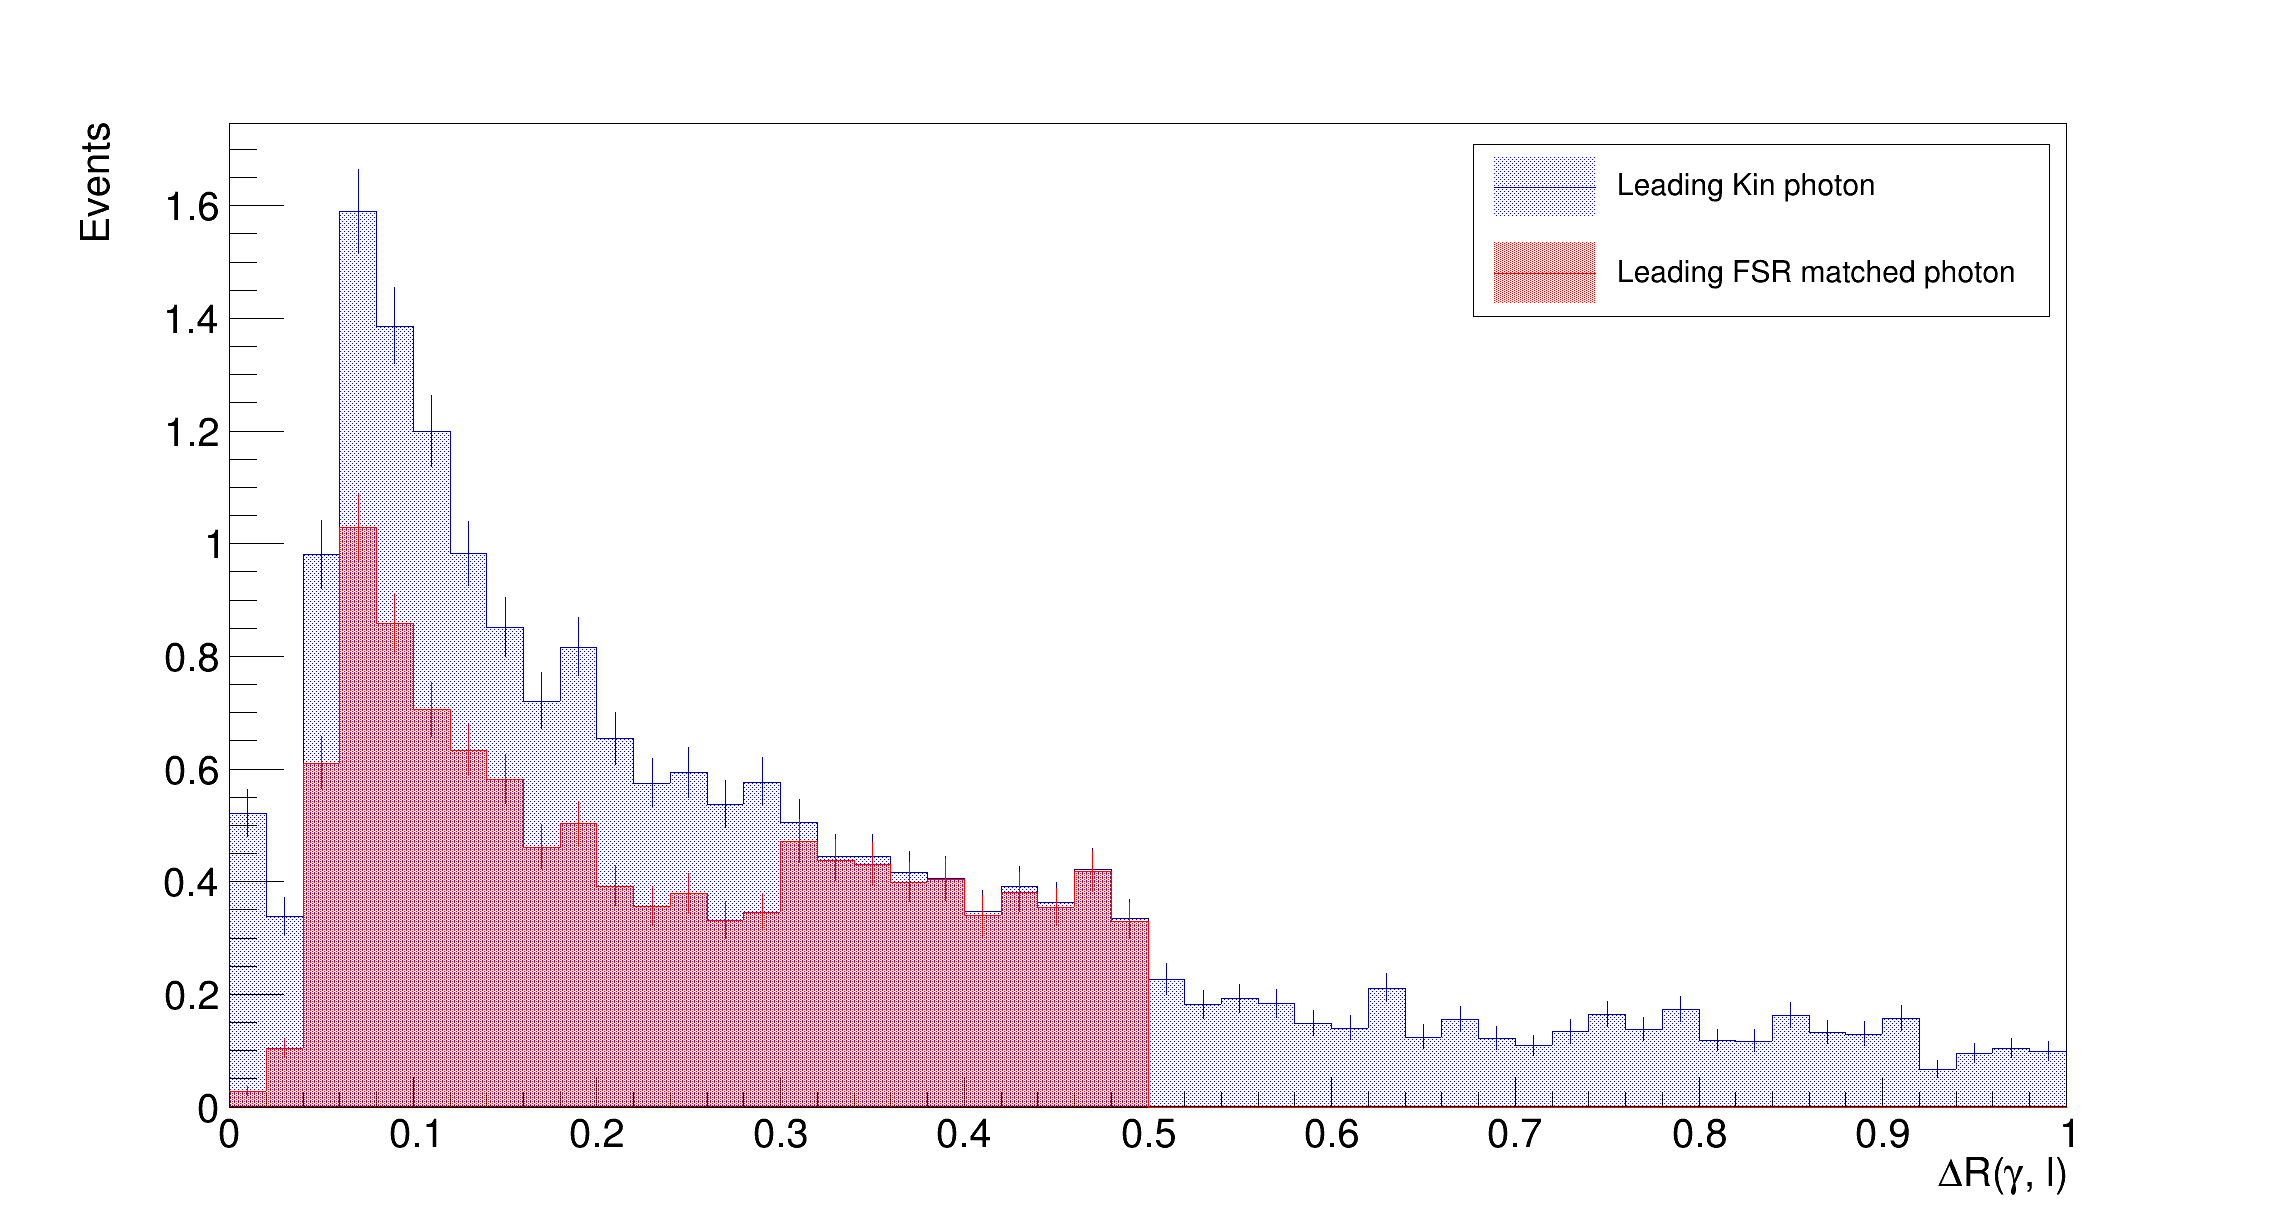
\includegraphics[width=0.8\textwidth]{Figures/lead_dRl_kin_vs_fsrMatched_rebinned.png}
\end{center}
\caption{$\Delta R(\ell, \gamma)$ for all the photons passing at least the `kinematic' selection with the $\Delta R$ cut relaxed, and for those selected as FSR in the ZZ$\gamma$ sample 2018.}
\label{fig:dRl_fsr_photons}
\end{figure}
% and the effect of not excluding FSR photons from the computation of the nonprompt rate
